\begin{apendicesenv}

\partapendices

\chapter{Processo}
\label{Processo}

\begin{figure}[h]
  \centering
  \label{fig01}
    \includegraphics[keepaspectratio=true, width=\textwidth]{figuras/ProcessoSAFE69.eps}
  \caption{Modelo do Projeto}
\end{figure}

\chapter{Documento de Visão}
\label{Visao}

{\large {\section { Histórico de Revisões \\ } } }


\begin{tabular}{|l|l|l|l|}
  \hline
  \textbf{Revisao} & Data &  Descricao &  Autor \\ \hline
  \textbf{0.1} &  17/10/2016 &  Versão Inicial &  Daniel, Miguel Nery \\ \hline
  \textbf{0.2} &  06/11/2016 &  Problema e Abordagem do Problema &  Daniel, Miguel Nery \\ \hline
  \textbf{0.3} &  14/11/2016 &  Abordagem dos Requisitos & Daniel, Eduardo \\ \hline
\end{tabular}

{\large {\section { Introdução \\ } } }

{\subsection {Finalidade\\ }}
Este documento contém os fatores mais relevantes que levarão à construção do site Chefe Nery. Esse projeto será desenvolvido pelos estudantes das disciplinas requisitos de software que é ministrada pela professora Elaine Venson da Universidade de Brasília, campus Gama/DF (FGA). Serão apresentadas aqui todas as principais características, finalidades e motivações para o desenvolvimento dessa aplicação, assim como as limitações e empecilhos que existem já na concepção da ideia.
\\

{\subsection {O problema\\ }}
\textbf{Discussão:} A fábrica de massas do Chefe Nery é uma micro-empresa que fornece produtos alimentícios em setores como culinária italiana, culinária oriental, entre outros. Realiza pedidos principalmente na Câmara dos Deputados, local de trabalho do dono da empresa e outras regiões próximas ao Plano Piloto e Park Way. Os pedidos são feitos majoritariamente pela plataforma mobile Whatsapp e com registros de pedidos não muito eficiente. \\
\tab \\
\textbf{Formulação do Problema:}


\newcommand{\nextitem}{\par\hspace*{\labelsep}\textbullet\hspace*{\labelsep}}

\begin{tabular}{|l|p{3in}|}
  \hline
  \textbf{O problema:} & \nextitem Pedidos feitos manualmente
    \nextitem Falta de divulgação da empresa
    \\ \hline
  \textbf{Afeta:} & \nextitem A gestão de pedidos
    \nextitem Estoque da empresa
    \\ \hline
  \textbf{Cujo impacto é:} & \nextitem Possível perda de pedidos
    \\ \hline
  \textbf{Uma boa solução seria:} & \nextitem Um sistema de plataforma web que realize os pedidos de forma autônoma e informasse à empresa sobre as entregas a serem feitas, além de informar aos clientes sobre os produtos preparados pelo chefe Nery.
    \\ \hline

\end{tabular}

{\large {\section { Abordagem do problema \\ } } }

\textbf{Discussão:} A fábrica de massas do Chefe Nery é uma micro-empresa que fornece produtos alimentícios em setores como culinária italiana, culinária oriental, entre outros. Realiza pedidos principalmente na Câmara dos Deputados, local de trabalho do dono da empresa e outras regiões próximas ao Plano Piloto e Park Way. Os pedidos são feitos majoritariamente pela plataforma mobile Whatsapp e com registros de pedidos não muito eficiente. \\

\textbf{Sentença de Posição do Produto:}  \\

\begin{tabular}{|l|p{3in}|}
  \hline
  \textbf{Para} & \nextitem Clientes que passam agora a pedir pelo sistema.
    \nextitem Administradores do estoque, uma vez o próprio sistema permite entregas caso haja estoque.
    \\ \hline
  \textbf{Que} & \nextitem Precisam realizar pedidos via internet
    \\ \hline
  \textbf{O produto} & \nextitem A aplicação do Chefe Nery
    \\ \hline
  \textbf{Faz} & \nextitem Expõe os produtos
  \nextitem Gerencia os pedidos
  \nextitem Cadastro de clientes
  \nextitem Realiza pagamentos (caso solicitado)
    \\ \hline

\end{tabular}
\tab \\ \\ \\
\large \textbf{Partes Envolvidas} \\
\tab \\ \\ \\
\textbf{Resumo dos Stakeholders:}  \\

\begin{tabular}{|p{1.5in}|p{1.6in}|p{1.7in}|}
  \hline
  \textbf{Nome} & \textbf{Descrição} & \textbf{Responsabilidades} \\ \hline
  Equipe de Desenvolvimento & Fazem parte do time de desenvolvedores & Responsáveis pela elaboração do programa \\ \hline
  Administradores & Quem administra o estoque e/ou pedidos & Responsável pela gerência de pedidos e estoques da empresa \\ \hline

\end{tabular} \\
\tab \\
\textbf{Resumo dos Usuários:}  \\

\begin{tabular}{|l|p{3in}|}
  \hline
  \textbf{Nome} & \textbf{Descrição} \\ \hline
  Clientes da fábrica de massas & Os clientes que irão fazer os pedidos pelo site \\ \hline
  Administradores & Os administradores da plataforma \\ \hline

\end{tabular}
\tab \\ \\
\textbf{Principais necessidades dos Usuários:} Os usuários necessitam de um canal que os possibilitem pesquisar os produtos existentes no site, escolher os produtos, assim como sua quantidade, o local de entrega dos produtos e identificar a forma de pagamento que julgarem necessária.   \\

{\large {\section { Perspectivas do Produto\\ } } }

\subsection{Descrição da Solução:}
Uma aplicação web para gerenciar pedidos, usuários e estoque e divulgar os produtos e meios de comunicação da microempresa Chef Nery. \\
\tab A aplicação tem como objetivo agilizar a comunicação entre compradores dos produtos Chef Nery e a microempresa Chef Nery, propriamente dita, além de divulgar seus produtos e facilitar seu controle de estoque e fluxo de caixa.\\
\tab O principal diferencial da aplicação é a  versatilidade de opções com que o administrador poderá: gerar relatórios de fluxo de caixa e visualizar o estado do estoque. Com tamanho controle do administrador, a tarefa de acompanhar a oscilações nos gastos e lucros torna-se menos cansativa e complicada.\\

\subsection{Benefícios do Produto:}
\subsubsection{Benefícios para o usuário:}
\begin{itemize}

\item Facilidade para visualizar e gerenciar compradores que estejam cadastrados no sistema.
\item Maior facilidade e praticidade para controlar estoque de produtos e fluxo de caixa.
\item Produtos e meios de comunicação mais amplamente divulgados.
\item Maior praticidade para receber pedidos.
\item Maior facilidade de conseguir novos compradores, ocasionais ou constantes.

\end{itemize}

\subsubsection{Benefícios para o administrador:}
\begin{itemize}

\item Maior praticidade para fazer pedidos de produtos Chef Nery.
\item Maior facilidade para conhecer os produtos Chef Nery e descobrir seus meios de comunicação.

\end{itemize}


{\large {\section { Principais Capacidades } } }

\begin{tabular}{|l|p{3in}|}
  \hline
  \textbf{Capacidade} & \textbf{Descrição} \\ \hline
  Expor produtos & Um Usuário ou Visitante poderá visualizar os produtos da empresa no estilo de um cardápio \\ \hline
  Expor meios de comunicação & Um Usuário ou Visitante poderá visualizar os endereços de comunicação da empresa \\ \hline
  Manter perfil de Usuário & Um Usuário pode cadastrar, atualizar e apagar seu perfil \\ \hline
  Visualização de fluxo de caixa & Os administradores da O Administrador poderá visualizar o fluxo de estoque registrado \\ \hline
  Pedido online & Um usuário poderá realizar pedidos inteiramente através do sistema \\ \hline

\end{tabular}
{\large {\section { Restrições do Projeto\\ } } }

O projeto é restringido pelo tempo e tamanho da equipe disponibilizados para sua conclusão.\\
\tab O projeto é restringido pela experiência dos integrantes da equipe em relação a gerência de requisitos, tópico que está sendo aprendido durante o tempo de desenvolvimento disponível.\\
{\large {\section { Atributos dos Requisitos\\ } } }

{\large {\subsection { Temas de Investimento\\ } } }


\textbf{TI1 - Gestão Administrativa} \\
\tab \\
\tab Data de criação do requisito: 12/11/2016;\\
\tab Início previsto: 13/11/2016;\\
\tab Término Previsto: Sem previsão;\\
\tab Valor para o negócio: Alto;\\
\tab Status do Requisito: Em progresso;\\
\tab Esforço: Planning Poker será jogado no início de cada sprint para determinar esforço.\\
\tab Descrição: Neste tema, a Gestão Administrativa cuida de cada aspecto da administração, sendo eles tanto de pedidos quanto de usuários e de produtos e envolve o épico Gestão de Pedidos. Nela é tratada todos os pontos que não são relativos ao marketing, que tem seu próprio tema de investimento.\\
\tab É dentro deste tema que serão definidas e aprimoradas cada atividade relacionada com a administração das informações relevantes para a efetivação da venda, relacionando os dados de usuários, produtos e pedidos automatizando toda a logística que anteriormente era realizada manualmente.\\
\\
\tab \\
\textbf{TI2 - Gestão de Marketing} \\
\tab \\
\tab Data de criação do requisito: 12/11/2016;\\
\tab Início previsto: 13/11/2016;\\
\tab Término Previsto: 17/11/2016;\\
\tab Valor para o negócio: Alto;\\
\tab Status do Requisito: Em progresso;\\
\tab Esforço: Planning Poker será jogado no início de cada sprint para determinar esforço.\\
\tab Descrição:  O tema de Gestão de Marketing inclui cada aspecto do sistema relativo a divulgação dos produtos e meios de comunicação da empresa Chef Nery.\\
\\

\textbf{Épicos} \\
\\
\textbf{EP1 - Gestão de Pedidos} \\ \\
\tab Data de criação do requisito: 12/11/2016;\\
\tab Início previsto: 13/11/2016;\\
\tab Término Previsto: Sem previsão;\\
\tab Valor para o negócio: Alto;\\
\tab Status do Requisito: Em progresso;\\
\tab Esforço: Planning Poker será jogado no início de cada sprint para determinar esforço.\\
\tab Descrição: A gestão dos pedidos consiste em um conjunto de funções relacionadas a informações sobre produtos que caracterizam ao que, como, quando e onde será entregue o pedido.\\
\\
\textbf{EP2 - Gestão de Marketing} \\ \\
\tab Data de criação do requisito: 12/11/2016;\\
\tab Início previsto: 13/11/2016;\\
\tab Término Previsto: 17/11/2016;\\
\tab Valor para o negócio: Alto;\\
\tab Status do Requisito: Em progresso;\\
\tab Esforço: Planning Poker será jogado no início de cada sprint para determinar esforço.\\
\tab Descrição:  A gestão da Exposição da Empresa consiste em um conjunto de atividades relacionadas com a comunicação entre a empresa e o seu cliente. Dentre estas atividades deve se destacar os planos de marketing.\\
\\

\textbf{Features} \\
\\
\textbf{FT1 - Sistema de Pedidos}\\ \\
\tab Data de criação do requisito: 12/11/2016;\\
\tab Início previsto: 13/11/2016;\\
\tab Término Previsto: Sem previsão;\\
\tab Valor para o negócio: Alto;\\
\tab Status do Requisito: Em progresso;\\
\tab Esforço: Planning Poker será jogado no início de cada sprint para determinar esforço.\\
\tab Descrição:  O sistema de pedidos do sistema deve efetuar o pedido de forma totalmente autônoma, integrado com o banco de dados do sistema e efetuar o pedido conforme o endereço passado pelo cliente com a forma de pagamento escolhida também por ele, tendo um feedback tanto para o cliente quanto para o administrador que recebe os pedidos.\\
\\
\textbf{FT2 - Gestão de Usuários}\\ \\
\tab Data de criação do requisito: 12/11/2016;\\
\tab Início previsto: 13/11/2016;\\
\tab Término Previsto: Sem previsão;\\
\tab Valor para o negócio: Alto;\\
\tab Status do Requisito: Em progresso;\\
\tab Esforço: Planning Poker será jogado no início de cada sprint para determinar esforço.\\
\tab Descrição:  Compradores são definidos segundo o tipo de pedidos que fazem:\\
\tab - Comprador Web: O usuário que faz pedidos pela plataforma web;\\
\tab - Comprador Direto: Aquele que compra diretamente com o Cliente;\\
\tab - Business to Business (BtoB): Empreendedores que compram grandes quantidades de produtos e os revende.\\
\\
\textbf{FT3 - Gestão de Produtos }\\ \\
\tab Data de criação do requisito: 12/11/2016;\\
\tab Início previsto: 13/11/2016;\\
\tab Término Previsto: Sem previsão;\\
\tab Valor para o negócio: Alto;\\
\tab Status do Requisito: Em progresso;\\
\tab Esforço: Planning Poker será jogado no início de cada sprint para determinar esforço.\\
\tab Descrição:  A Gestão de Produtos deve gerir os produtos envolvidos na Fábrica de Massas do Chef Nery, sendo integrado com o banco de dados do sistema. Além disso informar o valor de cada produto e gerar informações relevantes de acordo com o tempo acerca dos produtos.\\
\\
\textbf{FT4 - Divulgar Canais de Comunicação }\\ \\
\tab Data de criação do requisito: 12/11/2016;\\
\tab Início previsto: 13/11/2016;\\
\tab Término Previsto: 17/11/2016;\\
\tab Valor para o negócio: Alto;\\
\tab Status do Requisito: Em progresso;\\
\tab Esforço: Planning Poker será jogado no início de cada sprint para determinar esforço.\\
\tab Descrição: Disponibilizar informações do whatsapp e facebook da empresa a partir do site da empresa.\\
\\

\textbf{Histórias de Usuário}\\


\textbf{F1H1 - Pagar no ato da entrega }\\ \\
\tab Data de criação do requisito: 12/11/2016;\\
\tab Início previsto: Sem previsão;\\
\tab Término Previsto: Sem previsão;\\
\tab Valor para o negócio: Alto;\\
\tab Status do Requisito: Aberto;\\
\tab Esforço: Planning Poker será jogado no início de cada sprint para determinar esforço.\\
\tab Descrição: Eu como cliente desejo efetuar a compra, pegando somente na hora da entrega, a fim de pagar por dinheiro ou por cartão.\\
\\
\textbf{F1H2 - Pagar via sistema online}\\ \\
\tab Data de criação do requisito: 12/11/2016;\\
\tab Início previsto: Sem previsão;\\
\tab Término Previsto: Sem previsão;\\
\tab Valor para o negócio: Alto;\\
\tab Status do Requisito: Aberto;\\
\tab Esforço: Planning Poker será jogado no início de cada sprint para determinar esforço.\\
\tab Descrição: Eu como cliente desejo efetuar a compra e pagar por um sistema online(pagseguro), a fim de que o próprio sistema efetue o pagamento.\\
\\
\textbf{F1H3 - Efetuar pedido checando o estoque}\\ \\
\tab Data de criação do requisito: 12/11/2016;\\
\tab Início previsto: Sem previsão;\\
\tab Término Previsto: Sem previsão;\\
\tab Valor para o negócio: Alto;\\
\tab Status do Requisito: Aberto;\\
\tab Esforço: Planning Poker será jogado no início de cada sprint para determinar esforço.\\
\tab Descrição: Eu como administrador do estoque desejo que o próprio sistema avalie a ausência de produtos, a fim de permitir apenas pedidos com a possibilidade de entrega.\\
\\
\textbf{F1H4 - Escolher endereço de entrega}\\ \\
\tab Data de criação do requisito: 12/11/2016;\\
\tab Início previsto: Sem previsão;\\
\tab Término Previsto: Sem previsão;\\
\tab Valor para o negócio: Alto;\\
\tab Status do Requisito: Aberto;\\
\tab Esforço: Planning Poker será jogado no início de cada sprint para determinar esforço.\\
\tab Descrição: Eu como cliente desejo poder escolher o endereço de entrega a fim de que a entrega pode ser em um endereço cujo queira receber os pedidos (ambiente comercial, em domicílio, etc).\\
\\
\textbf{F1H5 - Ser alertado quanto a pedido}\\ \\
\tab Data de criação do requisito: 12/11/2016;\\
\tab Início previsto: Sem previsão;\\
\tab Término Previsto: Sem previsão;\\
\tab Valor para o negócio: Alto;\\
\tab Status do Requisito: Aberto;\\
\tab Esforço: Planning Poker será jogado no início de cada sprint para determinar esforço.\\
\tab Descrição: Eu como cliente e como vendedor desejo ser alertado quando o pedido foi efetuado para que tenha clareza quanto o status de aceitação do pedido.\\
\\
\textbf{F1H6 - Ajustar o preço conforme opção de entrega}\\ \\
\tab Data de criação do requisito: 12/11/2016;\\
\tab Início previsto: Sem previsão;\\
\tab Término Previsto: Sem previsão;\\
\tab Valor para o negócio: Alto;\\
\tab Status do Requisito: Aberto;\\
\tab Esforço: Planning Poker será jogado no início de cada sprint para determinar esforço.\\
\tab Descrição: Eu como administrador desejo que os preços sejam calculados de acordo com o local de entrega a fim de que o próprio sistema seja responsável pela conta do pagamento.\\
\\
\textbf{F2H1 - Cadastrar usuário}\\ \\
\tab Data de criação do requisito: 12/11/2016;\\
\tab Início previsto: 13/11/2016;\\
\tab Término Previsto: 17/11/2016;\\
\tab Valor para o negócio: Alto;\\
\tab Status do Requisito: Em progresso;\\
\tab Esforço: Planning Poker será jogado no início de cada sprint para determinar esforço.\\
\tab Descrição: Como Comprador, quero poder realizar meu cadastro no sistema para poder efetuar pedidos pela plataforma web.\\
\tab Compradores podem ser de diferentes tipos. Campos de cadastro devem exigir o mínimo que torne possível identificar o comprador (Quem, Onde, Contato).\\
\\
\textbf{F2H2 - Gerenciar conta}\\ \\
\tab Data de criação do requisito: 12/11/2016;\\
\tab Início previsto: Sem previsão;\\
\tab Término Previsto: Sem previsão;\\
\tab Valor para o negócio: Alto;\\
\tab Status do Requisito: Aberto;\\
\tab Esforço: Planning Poker será jogado no início de cada sprint para determinar esforço.\\
\tab Descrição: Como Comprador, quero poder gerenciar minha conta para poder visualizar ou atualizar meus dados ou apagar minha conta.\\
\\
\textbf{F2H3 Visualizar usuários}\\ \\
\tab Data de criação do requisito: 12/11/2016;\\
\tab Início previsto: Sem previsão;\\
\tab Término Previsto: Sem previsão;\\
\tab Valor para o negócio: Alto;\\
\tab Status do Requisito: Aberto;\\
\tab Esforço: Planning Poker será jogado no início de cada sprint para determinar esforço.\\
\tab Descrição: Como Administrador do sistema, preciso visualizar todos os usuários cadastrados para poder facilmente.\\
\\
\textbf{F3H1 - Manter Produto}\\ \\
\tab Data de criação do requisito: 12/11/2016;\\
\tab Início previsto: 15/11/2016;\\
\tab Término Previsto: 17/11/2016;\\
\tab Valor para o negócio: Alto;\\
\tab Status do Requisito: Em progresso;\\
\tab Esforço: Planning Poker será jogado no início de cada sprint para determinar esforço.\\
\tab Descrição: Como vendedor responsável pela Fábrica de Massas eu quero criar, atualizar, ler e deletar produtos para que seja possível ter um controle sobre quais e quantos produtos estão disponíveis no meu site.\\
\tab Será necessário identificar cada produto com as seguintes informações:\\
\tab - Nome do Produto;\\
\tab - Ingredientes;\\
\tab - Categoria (Culinária Italianas, Culinária Oriental, Culinária Árabe);\\
\tab - Preço do Produto;\\
\tab - Quantidade Disponível.\\
\\
\textbf{F3H2 - Calcular Valor do Produto}\\ \\
\tab Data de criação do requisito: 12/11/2016;\\
\tab Início previsto: Sem previsão;\\
\tab Término Previsto: Sem previsão;\\
\tab Valor para o negócio: Alto;\\
\tab Status do Requisito: Aberto;\\
\tab Esforço: Planning Poker será jogado no início de cada sprint para determinar esforço.\\
\tab Descrição: Como vendedor do produto desejo saber quanto custa cada produto baseado nos ingredientes e suas quantidades para que seja possível verificar o valor do produto. Esse custo será chamado de custo operacional.\\
\tab Opcionalmente, gostaria de saber o valor do produto baseado também no custo da gasolina do transporte para a entrega e também o próprio custo de tempo gasto pelo Chef Nery na produção do mesmo.\\
\\
\textbf{F3H3 - Gerar Relatório de Caixa}\\ \\
\tab Data de criação do requisito: 12/11/2016;\\
\tab Início previsto: Sem previsão;\\
\tab Término Previsto: Sem previsão;\\
\tab Valor para o negócio: Alto;\\
\tab Status do Requisito: Aberto;\\
\tab Esforço: Planning Poker será jogado no início de cada sprint para determinar esforço.\\
\tab Descrição: Como administrador da Fábrica de Massas quero saber a partir de um gráfico informações de acordo com o tempo acerca do fluxo de caixa de minha empresa envolvendo produtos vendidos para que seja possível ter um melhor controle da minha empresa. Devem ser disponibilizadas opções de visualização diária, semanal e anual.\\
\tab Opcionalmente com projeções futuras dos fluxos de caixa e a possibilidade de comparar fluxos de caixa.\\
\\
\textbf{F4H1 - Apresentar informações sobre a empresa e contatos}\\ \\
\tab Data de criação do requisito: 12/11/2016;\\
\tab Início previsto: 15/11/2016;\\
\tab Término Previsto: 17/11/2016;\\
\tab Valor para o negócio: Alto;\\
\tab Status do Requisito: Em progresso;\\
\tab Esforço: Planning Poker será jogado no início de cada sprint para determinar esforço.\\
\tab Descrição: Como vendedor responsável pela Fábrica de Massas eu quero disponibilizar informações para contato e atalhos para outros meios comunicação como facebook.\\
\tab Será necessário apresentar um atalho para a página oficial da empresa no Facebook e apresentar informações de contato como email e telefone.\\

\chapter{Especificação Suplementar}
\label{Suplementar}

{\large {\section { Introdução \\ } } }

Apesar do processos de desenvolvimento ter sido baseado no SAFe foi utilizado a especificação suplementar para definir o requisitos não funcionais. Desta forma, pode-se citar a definição de requisitos legais, reguladores, padrões de aplicação, de sistemas operacionais e ambiente, entre outros.

{\large {\section { Escopo \\ } } }

A fábrica de massas chefNery carece ainda de um site que otimize seu funcionamento. Assim, a equipe de requisitos tem como objetivos definir os requisitos da melhor forma possível e, possivelmente, implementar a aplicação conforme as necessidades e o interesse do cliente.

{\large {\section { Definições, Acrônimos e Abreviações \\ } } }

SAFe - (scaled agile Framework)

{\large {\section { Usabilidade \\ } } }

Estes requisitos foram desenvolvidos a partir das heurísticas e princípios de usabilidade.


\begin{table}[H]
                \centering
                \caption{Especificação dos Requisitos de Usabilidade}
                \begin{tabular}{c|p{10cm}}
                    \hline
                    \textbf{Requisito}            & \textbf{Descrição}\\
                    \hline
                    RU01 & A aplicação deverá ser de fácil aprendizado e compreensão por parte do usuário \\
                    \hline
                    RU02 & A aplicação deverá ser de fácil aprendizado e compreensão por parte do usuário \\
                    RU03 & A aplicação deve fornecer controle e liberdade ao usuário\\
                    \hline
                    RU04 & A aplicação deve apresentar consistência e padrões\\
                    \hline
                    RU05 & A aplicação deve prevenir erros por parte do usuário\\
                    \hline
                    RU06 & A aplicação deve apresentar ajuda e documentação de auxílio ao usuário\\
                    \hline
                \end{tabular}
            \end{table}


{\large {\section { Confiabilidade \\ } } }

\begin{table}[H]
                \centering
                \caption{Especificação dos Requisitos de Confiabilidade}
                \begin{tabular}{c|p{10cm}}
                    \hline
                    \textbf{Requisito}            & \textbf{Descrição}\\
                    \hline
                    RC01 & A aplicação deve garantir a privacidade dos dados dos clientes cadastrados\\
                    \hline
                    RC02 & A ocorrência de falhas deve ser a menor possível\\
                    \hline
                    RC03 & A aplicação deve possibilitar a recuperação dos dados\\
                    \hline
                    RC04 & A aplicação deve apresentar funcionamento estável\\
                    \hline
                \end{tabular}
            \end{table}


{\large {\section { Restrições do Design \\ } } }

\begin{table}[H]
                \centering
                \caption{Especificação dos Requisitos de Design}
                \begin{tabular}{c|p{10cm}}
                    \hline
                    \textbf{Requisito} & \textbf{Descrição}\\
                    \hline
                    RD01 & A Aplicação deverá fazer uso de Bootstrap\\
                    \hline
                    RD02 & A aplicação deverá utilizar recursos responsivos do bootstrap\\
                    \hline
                    RD03 & O repositório oficial da aplicação será o Github\\
                    \hline
                    RD04 & A arquitetura utilizada deve ser o MVC (model - view - controller)\\
                    \hline
                    RD05 &  A aplicação deverá ser feita a  partir da tecnologia ruby on rails\\
                    \hline
                \end{tabular}
            \end{table}

{\large {\section { Restrições do Sistema de Ajuda e Documentação de Usuário \\ } } }

A aplicação deverá apresentar documentação documentação de fácil visualização e disponibilidade. Esta poderá ser disponibilizada em uma página disponível dentro do site, fornecer um canal de comunicação e  até apresentar vídeos de manuseio do produto.\\

{\large {\section { Componentes adquiridos \\ } } }

A aplicação web necessita de um servidor e um domínio para sua hospedagem.\\

{\large {\section { Interfaces \\ } } }

{\subsection {Interfaces com o Usuário\\ }}

A interface do usuário deverá ser disponível para interação por meio de algum navegador web. Além disso, esta interface deverá ser responsiva.\\

{\subsection {Interfaces de Comunicação\\ }}

Para realizar a comunicação entre a aplicação e o dispositivos eletrônico será necessário o uso da internet.\\

{\large {\section { Observações Legais, copyright e Outros  \\ } } }

Esta aplicação se responsabiliza apenas para os critérios que foram definidos neste documento. Portanto, não é assegurado outros tópicos que não estão assegurados neste documento. \\

{\large {\section { Referências \\ } } }

Template Especificação Suplementar. UFPR. Disponível em: \href{http://www.funpar.ufpr.br:8080/rup/webtmpl/templates/req/rup_sspec.htm}{link}. Acesso em: 02 Novembro de 2016.\\

\chapter{Telas da Aplicação}
\begin{figure}[h]
    \centering
    \label{fig01}
        \includegraphics[keepaspectratio=true,scale=0.3]{figuras/SiteImagem1.eps}
    \caption{Home}
\end{figure}

\begin{figure}[h]
    \centering
    \label{fig01}
        \includegraphics[keepaspectratio=true,scale=0.3]{figuras/ImagemSobre.eps}
    \caption{Sobre}
\end{figure}

\begin{figure}[h]
    \centering
    \label{fig01}
        \includegraphics[keepaspectratio=true,scale=0.3]{figuras/ImagemContatos.eps}
    \caption{Contatos}
\end{figure}

\begin{figure}[h]
    \centering
    \label{fig01}
        \includegraphics[keepaspectratio=true,scale=0.3]{figuras/ImagemLogin.eps}
    \caption{Login}
\end{figure}

\begin{figure}[h]
    \centering
    \label{fig01}
        \includegraphics[keepaspectratio=true,scale=0.3]{figuras/ImagemCadastro.eps}
    \caption{Cadastro}
\end{figure}

\begin{figure}[h]
    \centering
    \label{fig01}
        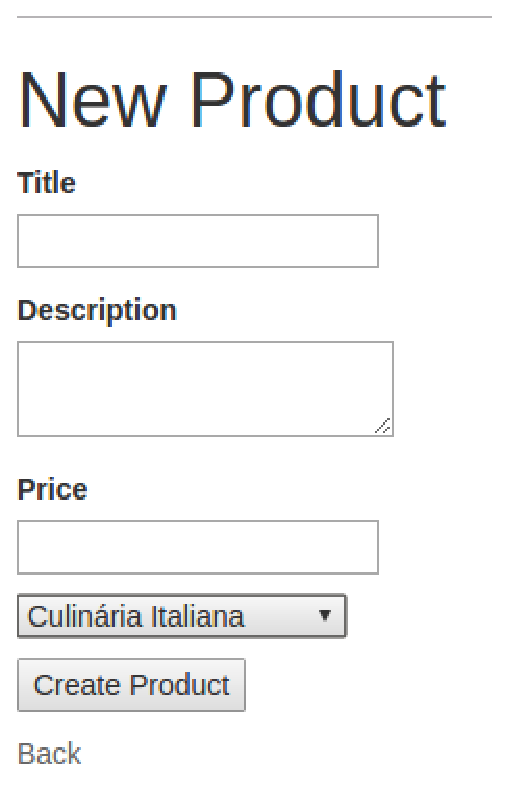
\includegraphics[keepaspectratio=true,scale=0.8]{figuras/NovoProduto.eps}
    \caption{Novo Produto}
\end{figure}

\chapter{Historico de Commits do Grupo}

\begin{figure}[h]
    \centering
    \label{fig01}
        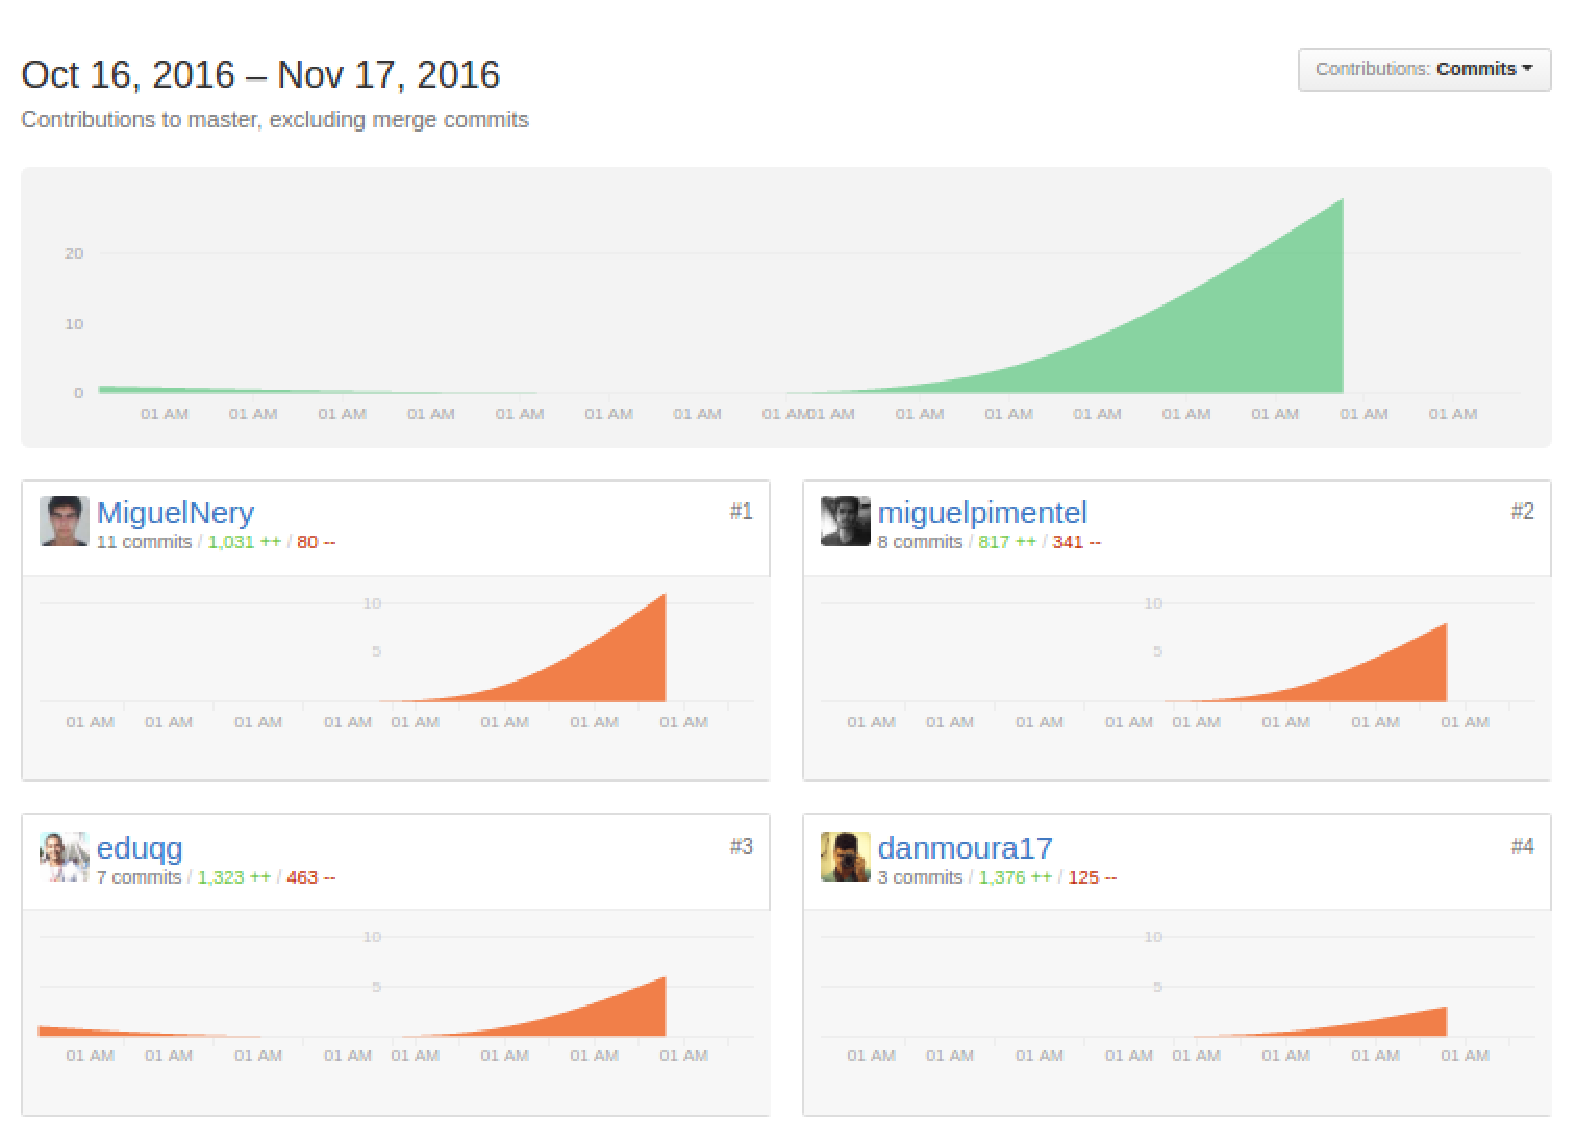
\includegraphics[keepaspectratio=true,scale=0.4]{figuras/ContribuicoesSite.eps}
    \caption{Contribuições do Site do Chef Nery}
\end{figure}

\begin{figure}[h]
    \centering
    \label{fig01}
        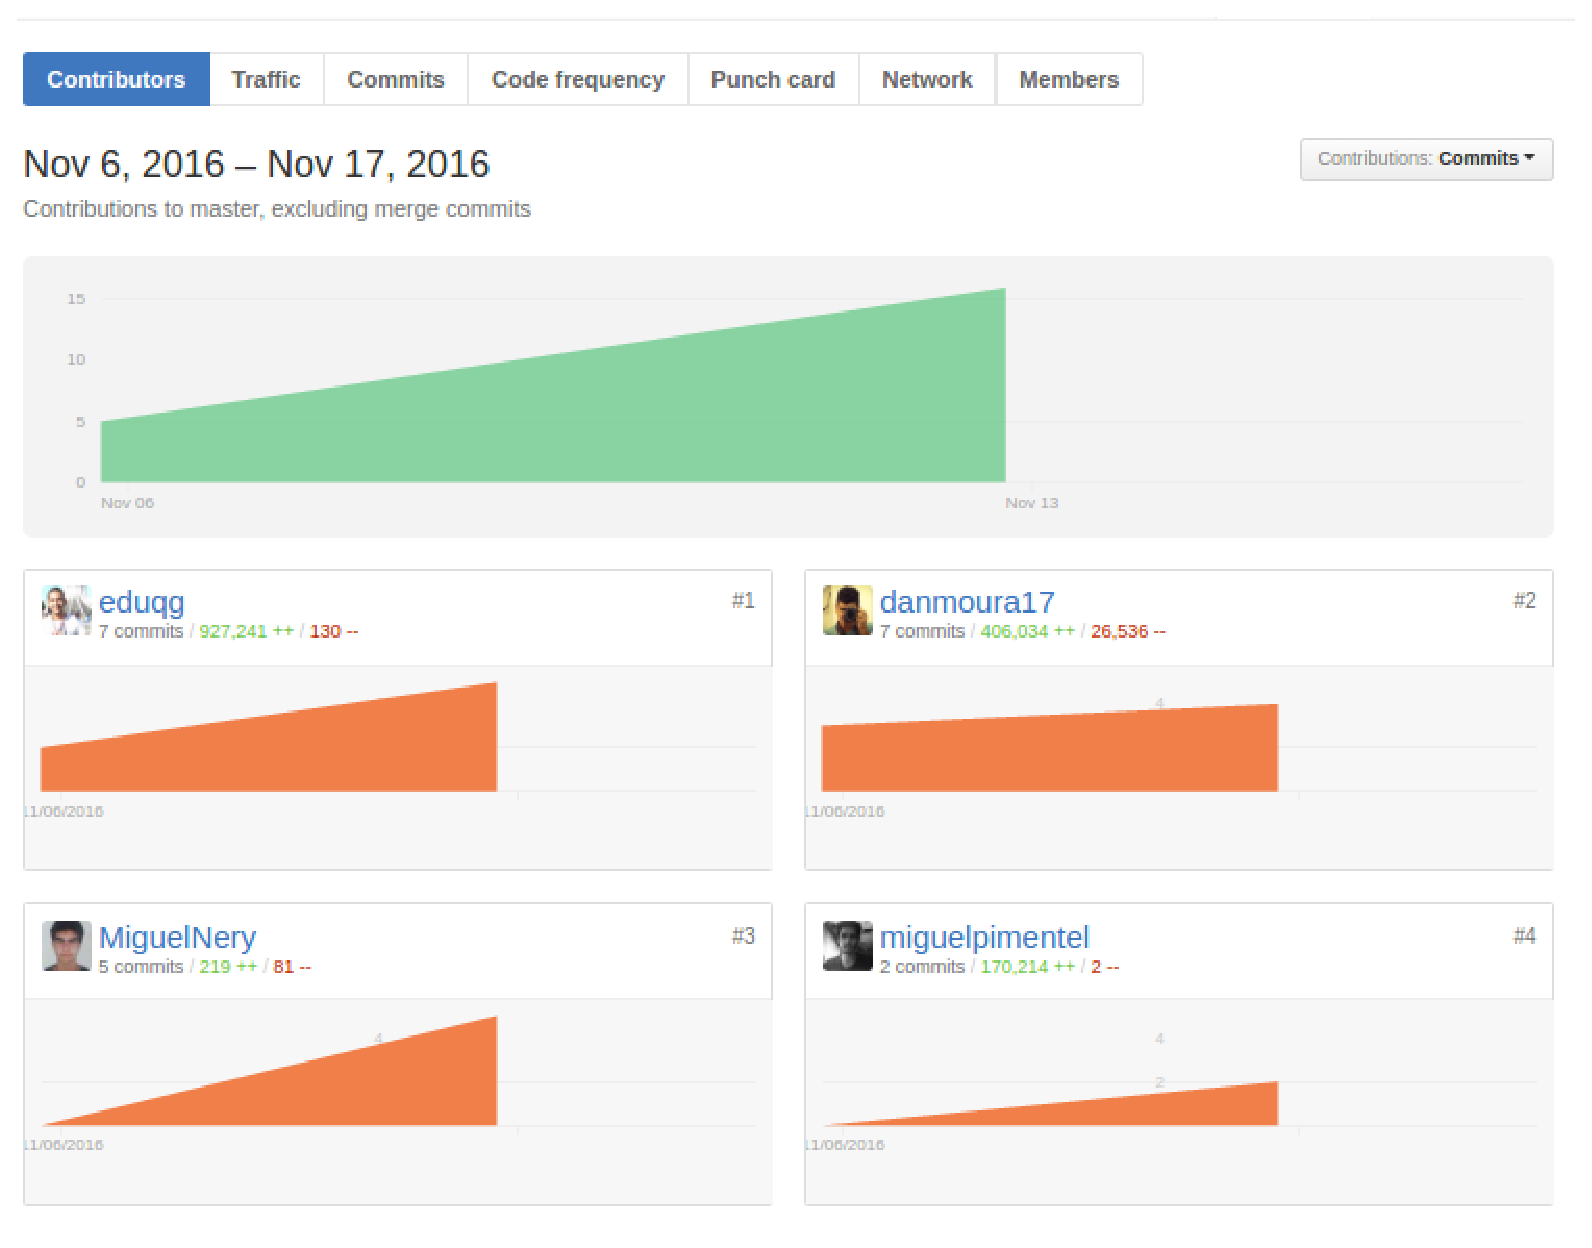
\includegraphics[keepaspectratio=true,scale=0.4]{figuras/ContribuicoesT2.eps}
    \caption{Contribuicoes Latex T2}
\end{figure}

\end{apendicesenv}
